\documentclass{article}
\usepackage{amsmath,amssymb,amsthm,enumitem} % Some standard math packages.
\usepackage{titling} % Enables \setlength{\droptitle}
\usepackage{parskip} % Cleaner paragraph display
\usepackage[margin=1in]{geometry} % Adjusts margins.
\usepackage[utf8]{inputenc} % USe UTF-8 input encoding instead of default ASCII.
\usepackage[]{forest} % Draws trees.
\usepackage{fancyvrb} % Allows Verbatim sections with line numbers and such. Note the capital V.
\usepackage{pgfplots}
\pgfplotsset{compat=1.6}
\newcommand {\todo}[1] {{\textbf{\color{red}#1}}}
\newcommand {code}[1] {\verb|#1|}

\title{CS 584 Research Project}
\author{ Dylan Laufenberg }
\date{June 5, 2018}

\begin{document}
\maketitle

\paragraph{Project topic} I will implement a variety of data structures that maintain total orders on their data, e.g. 2-3 trees, treaps, and skip lists; I will choose at least one deterministic structure as a reference and at least one randomized data structure for comparison. I will experimentally evaluate the rates of growth of their run times for insertions, searches, and deletions. Based on these data, I will discuss how the performance I observe compares to the predicted asymptotic performance.

\newpage
\section{Introduction}
This paper aims to illuminate various facets of the relationship between asymptotic complexity and empirical performance. The vehicle for this exploration is a series of benchmarks of data structures that perform similar jobs in very different ways. These include \todo{LIST OF DATA STRUCTURES}. For many tasks, they have the same asymptotic complexity, e.g. average complexity of $O(\log n)$ for search, insert, and delete operations, with worst-case complexity of $O(n)$ for each. This paper examines the performance characteristics of each and investigates how comparable the performance characteristics of these asymptotically equivalent data structures really are.

\section{Testing Methodology}

The core of the analysis in this paper is a collection of data sets gathered through benchmarking. Thus, it is essential to establish a reliable testing methodology, enforced through automation, to gather accurate data and ensure the integrity of the analysis that follows.

The test harness in 

\section{Data Structure Selection}
Many implementations exist for each of these data structures, since they are well-known. 


\newpage
\section{Testing TikZ Pictures}

\begin{figure}[h]
    \centering
    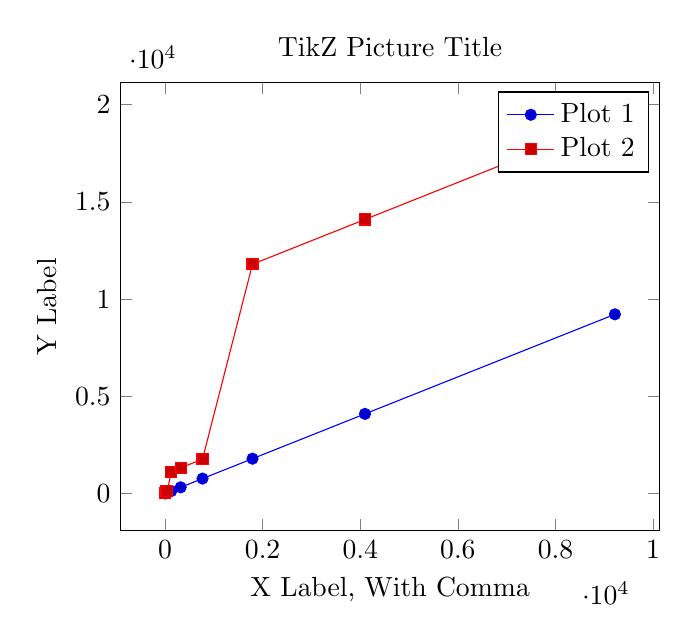
\begin{tikzpicture}
        \begin{axis}[xlabel={
            X Label, With Comma}, 
            ylabel=Y Label, 
            title=TikZ Picture Title
        ]
        \addplot coordinates {
            (5, 6)
            (17, 18)
            (49, 50)
            (129, 130)
            (321, 322)
            (769, 770)
            (1793, 1794)
            (4097, 4098)
            (9217, 9218)
        };
        \addplot coordinates {
            (5, 16)
            (17, 118)
            (49, 150)
            (129, 1130)
            (321, 1322)
            (769, 1770)
            (1793, 11794)
            (4097, 14098)
            (9217, 19218)
        };
        \legend{Plot 1, Plot 2}
        \end{axis}
    \end{tikzpicture}
    \caption{Figure Caption}
\end{figure}
\end{document}
